% !TeX spellcheck = en_US
\chapter{3D Computer Vision}
\label{cha:3D-cv}

\section{Introduction}
\label{sec:3D-cv-intro}
3D Computer Vision gives a representation that is closer of things that we interact in our lives. Thus, it will empower various novel applications in:
\begin{itemize}
	\item Autonomous Driving
	\item Robotics
	\item Remote Sensing
	\item Medical Treatment
	\item Design Industry
	\item Augmented Reality
\end{itemize}

\todo{} Learning resources: \href{https://??}{??}.

3D computer vision problems includes:
\begin{itemize}
	\item Depth extraction
	\item 3D Reconstruction
	\item Object Classification
	\item Object Detection
	\item Object Segmentation
	\item ??
\end{itemize}

Challenges of 3D computer vision:
\begin{itemize}
	\item something here
\end{itemize}

\section{Depth Extraction}
\hlb{The goal:} extract the depth, as the 3rd dimension for a 2D image.\\
The depth map is a simple grey image with values in range $[0, 255]$, $0$ for point afar and $255$ for points in near distances.
\begin{figure}[hbt!]
	\centering
	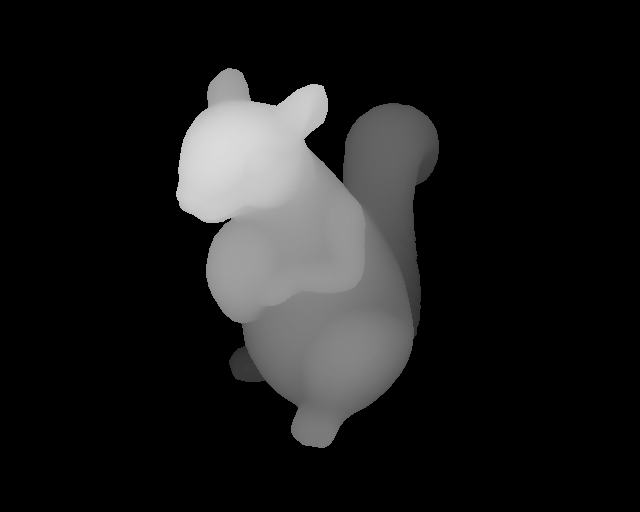
\includegraphics[width=0.57\textwidth]{depth-map.png}
	\caption{Example of a depth map \cite{tjaden2018}.}
\end{figure}

\section{3D Shape representation}
There are explicit representations and implicit representations, where parametric functions are used to differentiate a specific point is inside or outside the shape, or the distance to the shape surface. Typically, the parametric functions are in form of neural networks
\subsection{Voxel Grid}
\subsection{Point Cloud}
\subsection{Mesh}

\subsection{Occupancy}

\section{Classic 3D Reconstruction}
Geometric vision:
\begin{itemize}
	\item Visual Cues (Details)
	\begin{itemize}
		\item Shading
		\item Texture
		\item Focus
		\item Perspective
		\item Motion		
	\end{itemize}
	\item Stereo vision: process of extracting 3D information from multiple 2D views of a scene
\end{itemize}

\subsection{Epipolar Geometry}
Epipolar geometry is the geometry of stereo vision. The \hlr{basic principle} of epipolar geometry is \hlr{triangulation} of points.
\begin{figure}[hbt!]
	\centering
	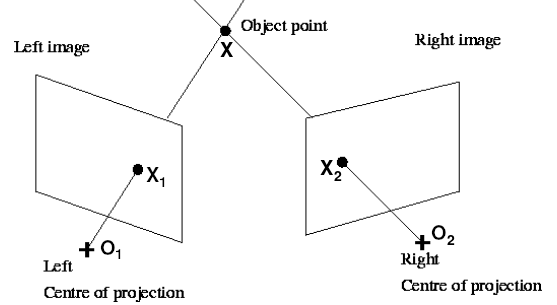
\includegraphics[width=0.57\textwidth]{triangulation.png}
	\caption{Example of triangulation (\href{https://homepages.inf.ed.ac.uk/rbf/CVonline/LOCAL_COPIES/OWENS/LECT10/node3.html}{src}). The lines connecting the camera poses with the correspondent points must intersect at the real object world space.}
	\label{fig:triangulation}
\end{figure}
In \figref{fig:triangulation}, $O_1$ and $O_2$ are the camera poses, $X_1$ and $X_2$ are the correspondent points on each image planes, and $X$ is the real object point in world space.

\todo{}

\subsection{Stereo Image Rectification}
Re-project image planes on to a common plane, which is parallel to the baseline\\
$\Rightarrow$ Scan lines are epipolar lines.

\todo{Add images}

\subsection{Correspondence Search}
Correspondence search simple means matching a point with another point in a different image.
\begin{table}[hbt!]
	\begin{tabularx}
		{\textwidth}{>{\setlength\hsize{\hsize}\setlength\linewidth{\hsize}}X|>{\setlength\hsize{\hsize}\setlength\linewidth{\hsize}}X}
		Dense Correspondence Search & Sparse Correspondence Search \\
		\hline
		\begin{itemize}
			\item For \hlr{each pixel}, find correspondence
			\item Easy when epipolar lines are scan lines (apply \hlr{rectification})
		\end{itemize} &
		\begin{itemize}
			\item Only for a set of detected feature
			\item Use feature description (Harris, SIFT??)
		\end{itemize}\\
		\multicolumn{2}{c}{------- \underline{Pros} -------}\\
		\begin{itemize}
			\item \hlr{Simple} process
			\item \hlr{More depth} $\Rightarrow$ useful for surface reconstruction
		\end{itemize} &
		\begin{itemize}
			\item \hlr{Efficiency}
			\item Can have more reliable matches
			\item Less sensitive to illumination $\Rightarrow$ \hlr{robust}
		\end{itemize}\\
		\multicolumn{2}{c}{------- \underline{Cons} -------}\\
		Problem with:
		\begin{itemize}
			\item \hlr{texture-less regions}
			\item different \hlr{viewpoints}
		\end{itemize} &
		\begin{itemize}
			\item Have to know enough to pick good features
			\item \hlr{Sparse} information
		\end{itemize}
	\end{tabularx}
\end{table}

\note \hlr{In practice, use both}.

\subsection{Stereo Reconstruction}
Main steps:
\begin{itemize}
	\item Calibrate cameras
	\item Rectify images
	\item Compute disparity
	\item Estimate depth
\end{itemize}
\hlr{This is just the \underline{ideal case}.}
\begin{itemize}
	\item What if, how can we get extrinsic \ac{info} from calibration?
	\item What to do when triangulation failed?
\end{itemize}

\subsection{Camera Calibration}
\subsection{Eight Point Algorithm}

\section{Deep Learning for 3D CV}

